\begin{appendices}
	%\newgeometry{top=0.7in,bottom=0.7in,left=1in,right=1in}
	
	\section*{mAP (mean Average Precision)}\label{appendix:mAP}
	
	\section*{IoU (Intersection over Union)}\label{appendix:IoU}
	L'IoU signifie Intersection over Union et est un calcul utilisé dans la technique de comparaison Pascal VOC.
	L'IoU est exprimé ainsi:
	$$\text{IoU} = \frac{\text{Aire de l'intersection}}{\text{Aire de l'union}}$$
	L'IoU, dans notre cas, ce calcul sur deux bounding box, comme dans la figure \ref{fig:iou_example}.
	\begin{figure}[!htbp]
	\center
		\subfloat{{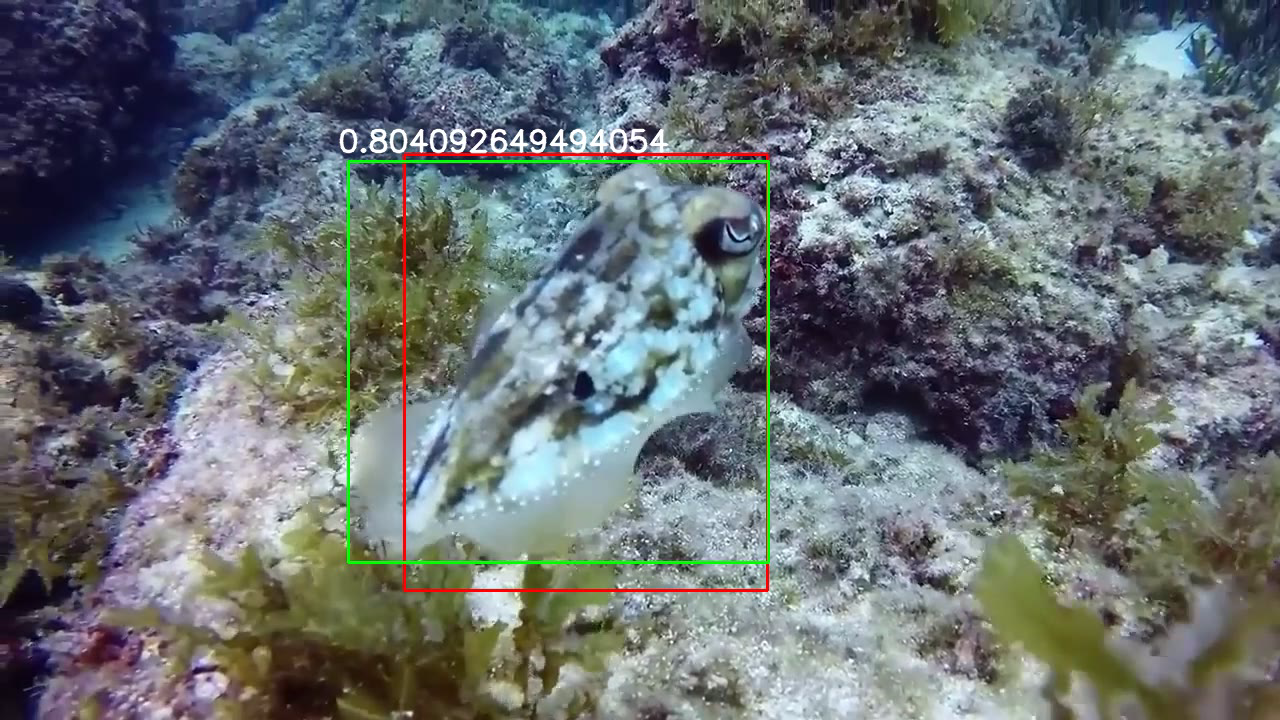
\includegraphics[scale=0.3]{eval0211.png}}}
	\caption{IoU (blanc) entre deux bounding box.}
	\label{fig:iou_example}
	\end{figure}
	\FloatBarrier
	
	\section*{Diagramme UML global}\label{appendix:UMLGlobal}
	\begin{figure}[!htbp]
		\center
			\subfloat{{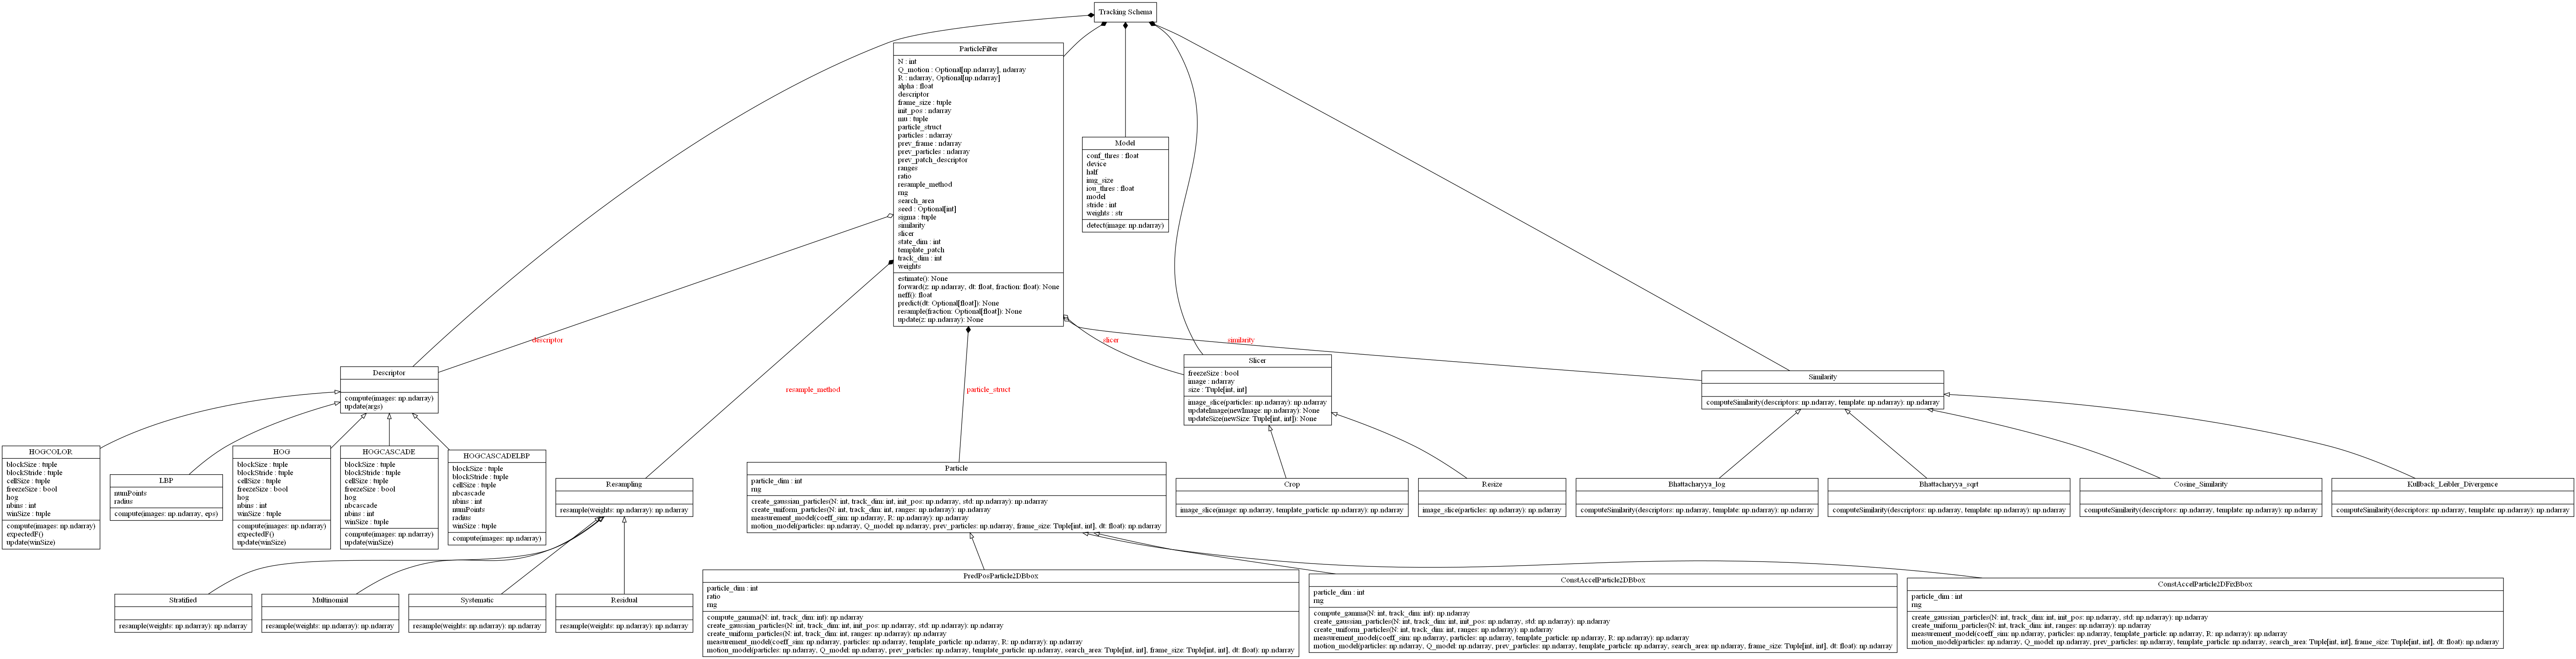
\includegraphics[scale=0.092,angle=90,origin=c]{classes.png}}}
		\caption{Diagramme UML des classes global.}
		\label{fig:uml_diagram_classes}
	\end{figure}
	\FloatBarrier
	
\end{appendices}

\clearpage